%package list
\documentclass{article}
\usepackage[top=3cm, bottom=3cm, outer=3cm, inner=3cm]{geometry}
\usepackage{multicol}
\usepackage{graphicx}
\usepackage{url}
%\usepackage{cite}
\usepackage{hyperref}
\usepackage{array}
%\usepackage{multicol}
\newcolumntype{x}[1]{>{\centering\arraybackslash\hspace{0pt}}p{#1}}
\usepackage{natbib}
\usepackage{pdfpages}
\usepackage{multirow}
\usepackage[normalem]{ulem}
\useunder{\uline}{\ul}{}
\usepackage{svg}
\usepackage{xcolor}
\usepackage{listings}
\lstdefinestyle{ascii-tree}{
    literate={├}{|}1 {─}{--}1 {└}{+}1 
  }
\lstset{basicstyle=\ttfamily,
  showstringspaces=false,
  commentstyle=\color{red},
  keywordstyle=\color{blue}
}
%\usepackage{booktabs}
\usepackage{caption}
\usepackage{subcaption}
\usepackage{float}
\usepackage{array}

\newcolumntype{M}[1]{>{\centering\arraybackslash}m{#1}}
\newcolumntype{N}{@{}m{0pt}@{}}


%%%%%%%%%%%%%%%%%%%%%%%%%%%%%%%%%%%%%%%%%%%%%%%%%%%%%%%%%%%%%%%%%%%%%%%%%%%%
%%%%%%%%%%%%%%%%%%%%%%%%%%%%%%%%%%%%%%%%%%%%%%%%%%%%%%%%%%%%%%%%%%%%%%%%%%%%
\newcommand{\itemEmail}{rvaldiviase@unsa.edu.pe}
\newcommand{\itemStudent}{Ryan Fabian Valdivia Segovia}
\newcommand{\itemCourse}{Fundamentos de la programación 2}
\newcommand{\itemCourseCode}{1701213}
\newcommand{\itemSemester}{II}
\newcommand{\itemUniversity}{Universidad Nacional de San Agustín de Arequipa}
\newcommand{\itemFaculty}{Facultad de Ingeniería de Producción y Servicios}
\newcommand{\itemDepartment}{Departamento Académico de Ingeniería de Sistemas e Informática}
\newcommand{\itemSchool}{Escuela Profesional de Ingeniería de Sistemas}
\newcommand{\itemAcademic}{2023 - B}
\newcommand{\itemInput}{Del 15 de Enero 2023}
\newcommand{\itemOutput}{Al 22 de Enero 2023}
\newcommand{\itemPracticeNumber}{22}
\newcommand{\itemTheme}{GUI : Interfaz Gráfica de Usuario}
%%%%%%%%%%%%%%%%%%%%%%%%%%%%%%%%%%%%%%%%%%%%%%%%%%%%%%%%%%%%%%%%%%%%%%%%%%%%
%%%%%%%%%%%%%%%%%%%%%%%%%%%%%%%%%%%%%%%%%%%%%%%%%%%%%%%%%%%%%%%%%%%%%%%%%%%%

\usepackage[english,spanish]{babel}
\usepackage[utf8]{inputenc}
\AtBeginDocument{\selectlanguage{spanish}}
\renewcommand{\figurename}{Figura}
\renewcommand{\refname}{Referencias}
\renewcommand{\tablename}{Tabla} %esto no funciona cuando se usa babel
\AtBeginDocument{%
	\renewcommand\tablename{Tabla}
}

\usepackage{fancyhdr}
\pagestyle{fancy}
\fancyhf{}
\setlength{\headheight}{30pt}
\renewcommand{\headrulewidth}{1pt}
\renewcommand{\footrulewidth}{1pt}
\fancyhead[L]{\raisebox{-0.2\height}{
\includegraphics[width=3cm]{img/logo_episunsa.png}}}
\fancyhead[C]{\fontsize{7}{7}\selectfont	\itemUniversity \\ \itemFaculty \\ \itemDepartment \\ \itemSchool \\ \textbf{\itemCourse}}
\fancyhead[R]{\raisebox{-0.2\height}{
\includegraphics[width=1.2cm]{img/logo_abet}}}
\fancyfoot[L]{Estudiante Ryan Valdivia}
\fancyfoot[C]{\itemCourse}
\fancyfoot[R]{Página \thepage}

% para el codigo fuente
\usepackage{listings}
\usepackage{color, colortbl}
\definecolor{dkgreen}{rgb}{0,0.6,0}
\definecolor{gray}{rgb}{0.5,0.5,0.5}
\definecolor{mauve}{rgb}{0.58,0,0.82}
\definecolor{codebackground}{rgb}{0.95, 0.95, 0.92}
\definecolor{tablebackground}{rgb}{0.8, 0, 0}

\lstset{frame=tb,
	language=bash,
	aboveskip=3mm,
	belowskip=3mm,
	showstringspaces=false,
	columns=flexible,
	basicstyle={\small\ttfamily},
	numbers=none,
	numberstyle=\tiny\color{gray},
	keywordstyle=\color{blue},
	commentstyle=\color{dkgreen},
	stringstyle=\color{mauve},
	breaklines=true,
	breakatwhitespace=true,
	tabsize=3,
	backgroundcolor= \color{codebackground},
}

\begin{document}
	
	\vspace*{10px}
	
	\begin{center}	
		\fontsize{17}{17} \textbf{ Informe de Laboratorio \itemPracticeNumber}
	\end{center}
	\centerline{\textbf{\Large Tema: \itemTheme}}
	%\vspace*{0.5cm}	

	\begin{flushright}
		\begin{tabular}{|M{2.5cm}|N|}
			\hline 
			\rowcolor{tablebackground}
			\color{white} \textbf{Nota}  \\
			\hline 
			     \\[30pt]
			\hline 			
		\end{tabular}
	\end{flushright}	

	\begin{table}[H]
		\begin{tabular}{|x{4.7cm}|x{4.8cm}|x{4.8cm}|}
			\hline 
			\rowcolor{tablebackground}
			\color{white} \textbf{Estudiante} & \color{white}\textbf{Escuela}  & \color{white}\textbf{Asignatura}   \\
			\hline 
			{\itemStudent \par \itemEmail} & \itemSchool & {\itemCourse \par Semestre: \itemSemester \par Código: \itemCourseCode}     \\
			\hline 			
		\end{tabular}
	\end{table}		
	
	\begin{table}[H]
		\begin{tabular}{|x{4.7cm}|x{4.8cm}|x{4.8cm}|}
			\hline 
			\rowcolor{tablebackground}
			\color{white}\textbf{Laboratorio} & \color{white}\textbf{Tema}  & \color{white}\textbf{Duración}   \\
			\hline 
			\itemPracticeNumber & \itemTheme & 04 horas   \\
			\hline 
		\end{tabular}
	\end{table}
	
	\begin{table}[H]
		\begin{tabular}{|x{4.7cm}|x{4.8cm}|x{4.8cm}|}
			\hline 
			\rowcolor{tablebackground}
			\color{white}\textbf{Semestre académico} & \color{white}\textbf{Fecha de inicio}  & \color{white}\textbf{Fecha de entrega}   \\
			\hline 
			\itemAcademic & \itemInput &  \itemOutput  \\
			\hline 
		\end{tabular}
	\end{table}
	
	\section{Tarea}
	\begin{itemize}
			\item Cree una versión del videojuego de estrategia usando componentes básicos GUI: Etiquetas, botones,
cuadros de texto, JOptionPane, Color.
			\item Además, utilizar componentes avanzados GUI: Layouts, JPanel, áreas de texto, checkbox, botones de
radio y combobox.
			\item Considerar nivel estratégico y táctico.
			\item Considerar hasta las unidades especiales de los reinos.
			\item Hacerlo iterativo.
	\end{itemize}
		
	\section{Equipos, materiales y temas utilizados}
	\begin{itemize}
		\item Sistema Operativo Windows 11 Home Single Language 64 bits 22621.2283
		\item VIM 9.0.
		\item Visual Studio Code 64 bits 1.82.2
		\item OpenJDK 64-Bits 21.0.2
		\item Git 2.41.0.windows.1
		\item IntelliJ IDEA 2023.3 Runtime version: 17.0.9+7-b1087.7 amd64
		\item Cuenta en GitHub con el correo institucional. 
	\end{itemize}
	
	\section{URL de Repositorio Github}
	\begin{itemize}
		\item URL del Repositorio GitHub para clonar o recuperar.
		\item \url{https://github.com/RyanValdivia/fp2-23b}
		\item URL para el laboratorio 22 en el Repositorio GitHub.
		\item \url{https://github.com/RyanValdivia/fp2-23b/tree/main/fase03/lab22}
	\end{itemize}
	
	\section{Actividades}
	\begin{itemize}	
		\item Este laboratorio consistía en elaborar una interfaz gráfica de usuario, portando todo nuestro videojuego de laboratorios anteriores.
		\item Para esto, reutilicé el código de laboratorios anteriores, usando la misma lógica. Entonces reciclé las clases de laboratorios anteriores
	\end{itemize}	
	\begin{lstlisting}[language=java,caption={Superclase Soldado}][H]
	package com.example.lab22;
import java.util.*;

public class Soldier {
    protected String name;
    protected String alias;
    protected int HP;
    protected int attack;
    protected int defense;
    protected int x;
    protected int y;
    protected boolean status;
    private String color;
    private int armyId;

    public Soldier(String name){
        this.name = name;
        this.status = true;
    }
    public Soldier(){
        this.name = "";
        this.alias = "";
        this.color = "#cdcdcd";
        this.status = false;
    }
   public void action(){};
    public static Soldier winner(Soldier s1, Soldier s2){
        Random random = new Random();
        double h1 = s1.getHP();
        double h2 = s2.getHP();
        double total = h1 + h2;
        h1 /= total;
        h2 /= total;
        double ans = random.nextDouble();
        if(h2 < h1){
            if(ans <= h2){
                return s2;
            }else{
                return s1;
            }
        }else{
            if(ans <= h1){
                return s1;
            }else{
                return s2;
            }
        }

    }
    public void copy(Soldier source){
        this.name = source.name;
        this.alias = source.alias;
        this.HP = source.HP;
        this.attack = source.attack;
        this.defense = source.defense;
        this.x = source.x;
        this.y = source.y;
        this.color = source.color;
        this.status = source.status;
        this.armyId = source.armyId;
    }
    public void destroy(){
        this.name = "";
        this.alias = "";
        this.HP = 0;
        this.attack = 0;
        this.defense = 0;
        this.status = false;
        this.color = "#cdcdcd";
        this.armyId = 0;
    }

    public String getName() {
        return name;
    }

    public void setName(String name) {
        this.name = name;
    }

    public String getAlias() {
        return alias;
    }

    public void setAlias(String alias) {
        this.alias = alias;
    }

    public int getHP() {
        return HP;
    }

    public void setHP(int HP) {
        this.HP = HP;
    }

    public int getAttack() {
        return attack;
    }

    public void setAttack(int attack) {
        this.attack = attack;
    }

    public int getDefense() {
        return defense;
    }

    public void setDefense(int defense) {
        this.defense = defense;
    }

    public int getX() {
        return x;
    }

    public String getColor() {
        return color;
    }

    public void setColor(String color) {
        this.color = color;
    }

    public int getArmyId() {
        return armyId;
    }

    public void setArmyId(int armyId) {
        this.armyId = armyId;
    }

    public void setX(int x) {
        this.x = x;
    }

    public int getY() {
        return y;
    }

    public void setY(int y) {
        this.y = y;
    }

    public boolean getStatus() {
        return status;
    }

    public void setStatus(boolean status) {
        this.status = status;
    }
}
class Archer extends Soldier{
    private int arrows;
    Random random = new Random();

    public Archer(String name) {
        super(name);
        this.arrows = random.nextInt(10);
        this.setAttack(7);
        this.setDefense(3);
        this.setHP(random.nextInt(3) + 3);
    }

    public int getArrows() {
        return arrows;
    }

    public void setArrows(int arrows) {
        this.arrows = arrows;
    }

    //Shoots one arrow to an enemy
    @Override
    public void action(){
        this.arrows--;
    }
}
class Knight extends Soldier{
    private String weapon;
    private boolean isMounted;
    Random random = new Random();

    public Knight(String name) {
        super(name);
        this.setAttack(13);
        this.setDefense(7);
        this.setHP(random.nextInt(3) + 10);
    }

    public String getWeapon() {
        return weapon;
    }

    public void setWeapon(String weapon) {
        this.weapon = weapon;
    }

    public boolean isMounted() {
        return isMounted;
    }

    public void setMounted(boolean mounted) {
        isMounted = mounted;
    }

    //If it's unmounted, it will mount and its weapon will change to a Sword, if not,
    // it will unmount and its weapon will change to a Spear
    @Override
    public void action(){
        this.isMounted = !this.isMounted;

        if(this.isMounted){
            this.weapon = "Sword";
        }else{
            this.weapon = "Spear";
        }
    }
}
class Swordsman extends Soldier{
    private final int swordLong;
    Random random = new Random();

    public Swordsman(String name) {
        super(name);
        this.swordLong = random.nextInt(10);
        this.setAttack(10);
        this.setDefense(8);
        this.setHP(random.nextInt(3) + 8);
    }

    public int getSwordLong() {
        return swordLong;
    }

    //This will set a wall of shields, and increase its defense by 1
    @Override
    public void action(){
        this.setDefense(this.getDefense() + 1);
    }
}
class Spearman extends Soldier{
    private final int spearLong;
    Random random = new Random();

    public Spearman(String name) {
        super(name);
        this.spearLong = random.nextInt(10);
        this.setAttack(5);
        this.setDefense(8);
        this.setHP(random.nextInt(3) + 8);
    }

    public int getSpearLong() {
        return spearLong;
    }

    //This will make a schiltrom and will increase its defense by 1
    @Override
    public void action(){
        this.setDefense(this.getDefense() + 1);
    }
}


	\end{lstlisting}
	\begin{itemize}	
		\item Es la misma clase de los laboratorios anteriores, solo que con pequeñas adaptaciones.
		\item Igual con las clases Army y Board (Mapa).
	\end{itemize}
	
	\begin{lstlisting}[language=java,caption={Clase Army}, numbers=left][H]
package com.example.lab22;
import java.util.*;
public class Army {
    private List<Soldier> soldiers = new ArrayList<>();
    private String[] realms = new String[]{
            "Inglaterra", "Francia", "Castilla-Aragon", "Moros", "Sacro Imperio Romano Germanico"
    };
    private String kingdom;
    private int id;
    private int nArchers = 0;
    private int nKnights = 0;
    private int nSwords = 0;
    private int nSpears = 0;


    Random random = new Random();

    public Army(int id) {
        this.kingdom = realms[random.nextInt(realms.length)];
        this.id = id;
        this.initialize();

    }
    public void initialize(){
        for (int i = 0; i < random.nextInt(10) + 1; i++) {
            switch (random.nextInt(4) + 1) {
                case 1:
                    Archer a = new Archer("Arquero" + i + "X" + id);
                    a.setAlias("A" + i + "X" + id);
                    a.setArmyId(id);
                    if(id == 1){
                        a.setColor("#b81414");
                    }else{
                        a.setColor("#00ffff");
                    }
                    nArchers++;
                    soldiers.add(a);
                    break;
                case 2:
                    Knight k = new Knight("Caballero" + i + "X" + id);
                    k.setAlias("C" + i + "X" + id);
                    k.setArmyId(id);
                    if(id == 1){
                        k.setColor("#b81414");
                    }else{
                        k.setColor("#00ffff");
                    }
                    nKnights++;
                    soldiers.add(k);
                    break;
                case 3:
                    Spearman s = new Spearman("Lancero" + i + "X" + id);
                    s.setAlias("L" + i + "X" + id);
                    s.setArmyId(id);
                    if(id == 1){
                        s.setColor("#b81414");
                    }else{
                        s.setColor("#00ffff");
                    }
                    nSpears++;
                    soldiers.add(s);
                    break;
                case 4:
                    Swordsman w = new Swordsman("Espadachin" + i + "X" + id);
                    w.setAlias("E" + i + "X" + id);
                    w.setArmyId(id);
                    if(id == 1){
                        w.setColor("#b81414");
                    }else{
                        w.setColor("#00ffff");
                    }
                    nSwords++;
                    soldiers.add(w);
                    break;
            }
        }
    }
    public void perk() {
        for (Soldier s : soldiers) {
            s.setHP(s.getHP() + 1);
        }
    }

    public List<Soldier> getSoldiers() {
        return soldiers;
    }

    public void setSoldiers(List<Soldier> soldiers) {
        this.soldiers = soldiers;
    }

    public String[] getRealms() {
        return realms;
    }

    public void setRealms(String[] realms) {
        this.realms = realms;
    }

    public String getKingdom() {
        return kingdom;
    }

    public void setKingdom(String kingdom) {
        this.kingdom = kingdom;
    }

    public int getId() {
        return id;
    }

    public void setId(int id) {
        this.id = id;
    }

    public int getnArchers() {
        return nArchers;
    }

    public void setnArchers(int nArchers) {
        this.nArchers = nArchers;
    }

    public int getnKnights() {
        return nKnights;
    }

    public void setnKnights(int nKnights) {
        this.nKnights = nKnights;
    }

    public int getnSwords() {
        return nSwords;
    }

    public void setnSwords(int nSwords) {
        this.nSwords = nSwords;
    }

    public int getnSpears() {
        return nSpears;
    }

    public void setnSpears(int nSpears) {
        this.nSpears = nSpears;
    }
}

	\end{lstlisting}
	
	\begin{lstlisting}[language=java,caption={Clase Board}, numbers=left][H]
package com.example.lab22;
import java.util.*;

public class Board {
    private Soldier[][] table = new Soldier[10][10];

    private String[] territories = new String[] {
            "Bosque", "Campo Abierto", "Montana", "Desierto", "Playa" };
    private String territory;
    private Map<String, String> perks = new HashMap<>();
    Random random = new Random();
    public Board() {
        this.territory = territories[random.nextInt(territories.length)];
    }
    public void initializeTable(){
        for(int i = 0; i < table.length; i++){
            for(int j = 0; j < table[i].length; j++){
                table[i][j] = new Soldier();
            }
        }
    }
    public void initializeArmy(Army a){
        for(Soldier s: a.getSoldiers()){
            int x = 0;
            int y = 0;
            do{
                x = random.nextInt(9);
                y = random.nextInt(9);
            }while(table[y][x].getStatus());
            s.setY(y);
            s.setX(x);
            table[y][x] = s;
        }
    }

    public Soldier[][] getTable() {
        return table;
    }

    public void setTable(Soldier[][] table) {
        this.table = table;
    }

    public String[] getTerritories() {
        return territories;
    }

    public void setTerritories(String[] territories) {
        this.territories = territories;
    }

    public String getTerritory() {
        return territory;
    }

    public void setTerritory(String territory) {
        this.territory = territory;
    }

    public Map<String, String> getPerks() {
        return perks;
    }

    public void setPerks(Map<String, String> perks) {
        this.perks = perks;
    }
}

	\end{lstlisting}
	\begin{itemize}
		\item Ahora si viene lo interesante, crear y aplicar la interfaz gráfica de usuario, para esto utilizaré JavaFX, usando IntelliJ IDEA como IDE, y SceneBuilder para realizar esto.
		\item Para comenzar el proyecto, creo una clase que implemente la interfaz gráfica en base a un archivo fxml, una clase que herede a la clase Application de JavaFx.
	\end{itemize}
	\begin{lstlisting}[language=java,caption={Clase HelloApplication}, numbers=left][H]
package com.example.lab22;

import javafx.application.Application;
import javafx.fxml.FXMLLoader;
import javafx.scene.Scene;
import javafx.stage.Stage;

import java.io.IOException;

public class HelloApplication extends Application {


    @Override
    public void start(Stage stage) throws IOException {
        FXMLLoader fxmlLoader = new FXMLLoader(HelloApplication.class.getResource("hello-view.fxml"));
        Scene scene = new Scene(fxmlLoader.load(), 670, 670);
        stage.setTitle("VideoJuego");
        stage.setScene(scene);
        stage.show();
    }

    public static void main(String[] args) {
        launch();
    }
}


	\end{lstlisting}
	
	\begin{itemize}	
		\item Esta clase implementa la interfaz gráfica en base a un fichero fxml, en el cual desarrollo lo que se va a mostrar al usuario.
		\item Para esta interfaz, decidí implementar 100 botones que representen un tablero de 10x10 usando el contenedor GridPane, para poder llevar una cuenta de las coordenadas de cada botón, además de una barra arriba del tablero para cambiar de turno, minimizar, cerrar o maximizar.
	\end{itemize}
	\begin{lstlisting}[language=java,caption={Archivo FXML}, numbers=left][H]
<?xml version="1.0" encoding="UTF-8"?>

<?import javafx.geometry.Insets?>
<?import javafx.scene.control.Button?>
<?import javafx.scene.layout.ColumnConstraints?>
<?import javafx.scene.layout.GridPane?>
<?import javafx.scene.layout.Pane?>
<?import javafx.scene.layout.RowConstraints?>
<?import javafx.scene.layout.VBox?>

<VBox fx:id="rootVBox" prefHeight="400.0" prefWidth="666.0" spacing="20.0" styleClass="vbox" stylesheets="@style.css" xmlns="http://javafx.com/javafx/21" xmlns:fx="http://javafx.com/fxml/1" fx:controller="com.example.lab22.HelloController">
    <padding>
        <Insets bottom="20.0" left="20.0" right="20.0" top="20.0" />
    </padding>
   <children>
      <Pane prefHeight="200.0" prefWidth="200.0" styleClass="toolBar">
         <children>
            <Pane fx:id="closeButton" layoutX="580.0" layoutY="-12.0" onMouseClicked="#handleCloseButton" />
             <Pane fx:id="minimizeButton" layoutX="520.0" layoutY="-12.0" onMouseClicked="#handleMinimizeButton" />
             <Pane fx:id="expandButton" layoutX="550.0" layoutY="-12.0" onMouseClicked="#handleExpandButton" />
             <Pane fx:id="nextButton" layoutX="15.0" layoutY="-12.0" onMouseClicked="#changeTurn" />
             <Pane fx:id="changeButton" />
         </children>
      </Pane>
       

      <GridPane id="board" fx:id="gridPane" prefHeight="330.0" prefWidth="352.0">
          <columnConstraints>
              <ColumnConstraints percentWidth="10" />
              <ColumnConstraints percentWidth="10" />
              <ColumnConstraints percentWidth="10" />
              <ColumnConstraints percentWidth="10" />
              <ColumnConstraints percentWidth="10" />
              <ColumnConstraints percentWidth="10" />
              <ColumnConstraints percentWidth="10" />
              <ColumnConstraints percentWidth="10" />
              <ColumnConstraints percentWidth="10" />
              <ColumnConstraints percentWidth="10" />
          </columnConstraints>
          <rowConstraints>
              <RowConstraints percentHeight="10" vgrow="SOMETIMES" />
              <RowConstraints percentHeight="10" vgrow="SOMETIMES" />
              <RowConstraints percentHeight="10" vgrow="SOMETIMES" />
              <RowConstraints percentHeight="10" vgrow="SOMETIMES" />
              <RowConstraints percentHeight="10" vgrow="SOMETIMES" />
              <RowConstraints percentHeight="10" vgrow="SOMETIMES" />
              <RowConstraints percentHeight="10" vgrow="SOMETIMES" />
              <RowConstraints percentHeight="10" vgrow="SOMETIMES" />
              <RowConstraints percentHeight="10" vgrow="SOMETIMES" />
              <RowConstraints percentHeight="10" vgrow="SOMETIMES" />
          </rowConstraints>
         <children>

             <!-- Row 0 -->
             <Button mnemonicParsing="false" onMouseClicked="#onButtonClick" styleClass="button" text="" GridPane.columnIndex="0" GridPane.rowIndex="0" />
             <Button mnemonicParsing="false" onMouseClicked="#onButtonClick" styleClass="button" text="" GridPane.columnIndex="1" GridPane.rowIndex="0" />
             <Button mnemonicParsing="false" onMouseClicked="#onButtonClick" styleClass="button" text="" GridPane.columnIndex="2" GridPane.rowIndex="0" />
             <Button mnemonicParsing="false" onMouseClicked="#onButtonClick" styleClass="button" text="" GridPane.columnIndex="3" GridPane.rowIndex="0" />
             <Button mnemonicParsing="false" onMouseClicked="#onButtonClick" styleClass="button" text="" GridPane.columnIndex="4" GridPane.rowIndex="0" />
             <Button mnemonicParsing="false" onMouseClicked="#onButtonClick" styleClass="button" text="" GridPane.columnIndex="5" GridPane.rowIndex="0" />
             <Button mnemonicParsing="false" onMouseClicked="#onButtonClick" styleClass="button" text="" GridPane.columnIndex="6" GridPane.rowIndex="0" />
             <Button mnemonicParsing="false" onMouseClicked="#onButtonClick" styleClass="button" text="" GridPane.columnIndex="7" GridPane.rowIndex="0" />
             <Button mnemonicParsing="false" onMouseClicked="#onButtonClick" styleClass="button" text="" GridPane.columnIndex="8" GridPane.rowIndex="0" />
             <Button mnemonicParsing="false" onMouseClicked="#onButtonClick" styleClass="button" text="" GridPane.columnIndex="9" GridPane.rowIndex="0" />

             <!-- Row 1 -->
             <Button mnemonicParsing="false" onMouseClicked="#onButtonClick" styleClass="button" text="" GridPane.columnIndex="0" GridPane.rowIndex="1" />
             <Button mnemonicParsing="false" onMouseClicked="#onButtonClick" styleClass="button" text="" GridPane.columnIndex="1" GridPane.rowIndex="1" />
             <Button mnemonicParsing="false" onMouseClicked="#onButtonClick" styleClass="button" text="" GridPane.columnIndex="2" GridPane.rowIndex="1" />
             <Button mnemonicParsing="false" onMouseClicked="#onButtonClick" styleClass="button" text="" GridPane.columnIndex="3" GridPane.rowIndex="1" />
             <Button mnemonicParsing="false" onMouseClicked="#onButtonClick" styleClass="button" text="" GridPane.columnIndex="4" GridPane.rowIndex="1" />
             <Button mnemonicParsing="false" onMouseClicked="#onButtonClick" styleClass="button" text="" GridPane.columnIndex="5" GridPane.rowIndex="1" />
             <Button mnemonicParsing="false" onMouseClicked="#onButtonClick" styleClass="button" text="" GridPane.columnIndex="6" GridPane.rowIndex="1" />
             <Button mnemonicParsing="false" onMouseClicked="#onButtonClick" styleClass="button" text="" GridPane.columnIndex="7" GridPane.rowIndex="1" />
             <Button mnemonicParsing="false" onMouseClicked="#onButtonClick" styleClass="button" text="" GridPane.columnIndex="8" GridPane.rowIndex="1" />
             <Button mnemonicParsing="false" onMouseClicked="#onButtonClick" styleClass="button" text="" GridPane.columnIndex="9" GridPane.rowIndex="1" />

             <!-- Row 2 -->
             <Button mnemonicParsing="false" onMouseClicked="#onButtonClick" styleClass="button" text="" GridPane.columnIndex="0" GridPane.rowIndex="2" />
             <Button mnemonicParsing="false" onMouseClicked="#onButtonClick" styleClass="button" text="" GridPane.columnIndex="1" GridPane.rowIndex="2" />
             <Button mnemonicParsing="false" onMouseClicked="#onButtonClick" styleClass="button" text="" GridPane.columnIndex="2" GridPane.rowIndex="2" />
             <Button mnemonicParsing="false" onMouseClicked="#onButtonClick" styleClass="button" text="" GridPane.columnIndex="3" GridPane.rowIndex="2" />
             <Button mnemonicParsing="false" onMouseClicked="#onButtonClick" styleClass="button" text="" GridPane.columnIndex="4" GridPane.rowIndex="2" />
             <Button mnemonicParsing="false" onMouseClicked="#onButtonClick" styleClass="button" text="" GridPane.columnIndex="5" GridPane.rowIndex="2" />
             <Button mnemonicParsing="false" onMouseClicked="#onButtonClick" styleClass="button" text="" GridPane.columnIndex="6" GridPane.rowIndex="2" />
             <Button mnemonicParsing="false" onMouseClicked="#onButtonClick" styleClass="button" text="" GridPane.columnIndex="7" GridPane.rowIndex="2" />
             <Button mnemonicParsing="false" onMouseClicked="#onButtonClick" styleClass="button" text="" GridPane.columnIndex="8" GridPane.rowIndex="2" />
             <Button mnemonicParsing="false" onMouseClicked="#onButtonClick" styleClass="button" text="" GridPane.columnIndex="9" GridPane.rowIndex="2" />

             <!-- Row 3 -->
             <Button mnemonicParsing="false" onMouseClicked="#onButtonClick" styleClass="button" text="" GridPane.columnIndex="0" GridPane.rowIndex="3" />
             <Button mnemonicParsing="false" onMouseClicked="#onButtonClick" styleClass="button" text="" GridPane.columnIndex="1" GridPane.rowIndex="3" />
             <Button mnemonicParsing="false" onMouseClicked="#onButtonClick" styleClass="button" text="" GridPane.columnIndex="2" GridPane.rowIndex="3" />
             <Button mnemonicParsing="false" onMouseClicked="#onButtonClick" styleClass="button" text="" GridPane.columnIndex="3" GridPane.rowIndex="3" />
             <Button mnemonicParsing="false" onMouseClicked="#onButtonClick" styleClass="button" text="" GridPane.columnIndex="4" GridPane.rowIndex="3" />
             <Button mnemonicParsing="false" onMouseClicked="#onButtonClick" styleClass="button" text="" GridPane.columnIndex="5" GridPane.rowIndex="3" />
             <Button mnemonicParsing="false" onMouseClicked="#onButtonClick" styleClass="button" text="" GridPane.columnIndex="6" GridPane.rowIndex="3" />
             <Button mnemonicParsing="false" onMouseClicked="#onButtonClick" styleClass="button" text="" GridPane.columnIndex="7" GridPane.rowIndex="3" />
             <Button mnemonicParsing="false" onMouseClicked="#onButtonClick" styleClass="button" text="" GridPane.columnIndex="8" GridPane.rowIndex="3" />
             <Button mnemonicParsing="false" onMouseClicked="#onButtonClick" styleClass="button" text="" GridPane.columnIndex="9" GridPane.rowIndex="3" />

             <!-- Row 4 -->
             <Button mnemonicParsing="false" onMouseClicked="#onButtonClick" styleClass="button" text="" GridPane.columnIndex="0" GridPane.rowIndex="4" />
             <Button mnemonicParsing="false" onMouseClicked="#onButtonClick" styleClass="button" text="" GridPane.columnIndex="1" GridPane.rowIndex="4" />
             <Button mnemonicParsing="false" onMouseClicked="#onButtonClick" styleClass="button" text="" GridPane.columnIndex="2" GridPane.rowIndex="4" />
             <Button mnemonicParsing="false" onMouseClicked="#onButtonClick" styleClass="button" text="" GridPane.columnIndex="3" GridPane.rowIndex="4" />
             <Button mnemonicParsing="false" onMouseClicked="#onButtonClick" styleClass="button" text="" GridPane.columnIndex="4" GridPane.rowIndex="4" />
             <Button mnemonicParsing="false" onMouseClicked="#onButtonClick" styleClass="button" text="" GridPane.columnIndex="5" GridPane.rowIndex="4" />
             <Button mnemonicParsing="false" onMouseClicked="#onButtonClick" styleClass="button" text="" GridPane.columnIndex="6" GridPane.rowIndex="4" />
             <Button mnemonicParsing="false" onMouseClicked="#onButtonClick" styleClass="button" text="" GridPane.columnIndex="7" GridPane.rowIndex="4" />
             <Button mnemonicParsing="false" onMouseClicked="#onButtonClick" styleClass="button" text="" GridPane.columnIndex="8" GridPane.rowIndex="4" />
             <Button mnemonicParsing="false" onMouseClicked="#onButtonClick" styleClass="button" text="" GridPane.columnIndex="9" GridPane.rowIndex="4" />

             <!-- Row 5 -->
             <Button mnemonicParsing="false" onMouseClicked="#onButtonClick" styleClass="button" text="" GridPane.columnIndex="0" GridPane.rowIndex="5" />
             <Button mnemonicParsing="false" onMouseClicked="#onButtonClick" styleClass="button" text="" GridPane.columnIndex="1" GridPane.rowIndex="5" />
             <Button mnemonicParsing="false" onMouseClicked="#onButtonClick" styleClass="button" text="" GridPane.columnIndex="2" GridPane.rowIndex="5" />
             <Button mnemonicParsing="false" onMouseClicked="#onButtonClick" styleClass="button" text="" GridPane.columnIndex="3" GridPane.rowIndex="5" />
             <Button mnemonicParsing="false" onMouseClicked="#onButtonClick" styleClass="button" text="" GridPane.columnIndex="4" GridPane.rowIndex="5" />
             <Button mnemonicParsing="false" onMouseClicked="#onButtonClick" styleClass="button" text="" GridPane.columnIndex="5" GridPane.rowIndex="5" />
             <Button mnemonicParsing="false" onMouseClicked="#onButtonClick" styleClass="button" text="" GridPane.columnIndex="6" GridPane.rowIndex="5" />
             <Button mnemonicParsing="false" onMouseClicked="#onButtonClick" styleClass="button" text="" GridPane.columnIndex="7" GridPane.rowIndex="5" />
             <Button mnemonicParsing="false" onMouseClicked="#onButtonClick" styleClass="button" text="" GridPane.columnIndex="8" GridPane.rowIndex="5" />
             <Button mnemonicParsing="false" onMouseClicked="#onButtonClick" styleClass="button" text="" GridPane.columnIndex="9" GridPane.rowIndex="5" />

             <!-- Row 6 -->
             <Button mnemonicParsing="false" onMouseClicked="#onButtonClick" styleClass="button" text="" GridPane.columnIndex="0" GridPane.rowIndex="6" />
             <Button mnemonicParsing="false" onMouseClicked="#onButtonClick" styleClass="button" text="" GridPane.columnIndex="1" GridPane.rowIndex="6" />
             <Button mnemonicParsing="false" onMouseClicked="#onButtonClick" styleClass="button" text="" GridPane.columnIndex="2" GridPane.rowIndex="6" />
             <Button mnemonicParsing="false" onMouseClicked="#onButtonClick" styleClass="button" text="" GridPane.columnIndex="3" GridPane.rowIndex="6" />
             <Button mnemonicParsing="false" onMouseClicked="#onButtonClick" styleClass="button" text="" GridPane.columnIndex="4" GridPane.rowIndex="6" />
             <Button mnemonicParsing="false" onMouseClicked="#onButtonClick" styleClass="button" text="" GridPane.columnIndex="5" GridPane.rowIndex="6" />
             <Button mnemonicParsing="false" onMouseClicked="#onButtonClick" styleClass="button" text="" GridPane.columnIndex="6" GridPane.rowIndex="6" />
             <Button mnemonicParsing="false" onMouseClicked="#onButtonClick" styleClass="button" text="" GridPane.columnIndex="7" GridPane.rowIndex="6" />
             <Button mnemonicParsing="false" onMouseClicked="#onButtonClick" styleClass="button" text="" GridPane.columnIndex="8" GridPane.rowIndex="6" />
             <Button mnemonicParsing="false" onMouseClicked="#onButtonClick" styleClass="button" text="" GridPane.columnIndex="9" GridPane.rowIndex="6" />

             <!-- Row 7 -->
             <Button mnemonicParsing="false" onMouseClicked="#onButtonClick" styleClass="button" text="" GridPane.columnIndex="0" GridPane.rowIndex="7" />
             <Button mnemonicParsing="false" onMouseClicked="#onButtonClick" styleClass="button" text="" GridPane.columnIndex="1" GridPane.rowIndex="7" />
             <Button mnemonicParsing="false" onMouseClicked="#onButtonClick" styleClass="button" text="" GridPane.columnIndex="2" GridPane.rowIndex="7" />
             <Button mnemonicParsing="false" onMouseClicked="#onButtonClick" styleClass="button" text="" GridPane.columnIndex="3" GridPane.rowIndex="7" />
             <Button mnemonicParsing="false" onMouseClicked="#onButtonClick" styleClass="button" text="" GridPane.columnIndex="4" GridPane.rowIndex="7" />
             <Button mnemonicParsing="false" onMouseClicked="#onButtonClick" styleClass="button" text="" GridPane.columnIndex="5" GridPane.rowIndex="7" />
             <Button mnemonicParsing="false" onMouseClicked="#onButtonClick" styleClass="button" text="" GridPane.columnIndex="6" GridPane.rowIndex="7" />
             <Button mnemonicParsing="false" onMouseClicked="#onButtonClick" styleClass="button" text="" GridPane.columnIndex="7" GridPane.rowIndex="7" />
             <Button mnemonicParsing="false" onMouseClicked="#onButtonClick" styleClass="button" text="" GridPane.columnIndex="8" GridPane.rowIndex="7" />
             <Button mnemonicParsing="false" onMouseClicked="#onButtonClick" styleClass="button" text="" GridPane.columnIndex="9" GridPane.rowIndex="7" />

             <!-- Row 8 -->
             <Button mnemonicParsing="false" onMouseClicked="#onButtonClick" styleClass="button" text="" GridPane.columnIndex="0" GridPane.rowIndex="8" />
             <Button mnemonicParsing="false" onMouseClicked="#onButtonClick" styleClass="button" text="" GridPane.columnIndex="1" GridPane.rowIndex="8" />
             <Button mnemonicParsing="false" onMouseClicked="#onButtonClick" styleClass="button" text="" GridPane.columnIndex="2" GridPane.rowIndex="8" />
             <Button mnemonicParsing="false" onMouseClicked="#onButtonClick" styleClass="button" text="" GridPane.columnIndex="3" GridPane.rowIndex="8" />
             <Button mnemonicParsing="false" onMouseClicked="#onButtonClick" styleClass="button" text="" GridPane.columnIndex="4" GridPane.rowIndex="8" />
             <Button mnemonicParsing="false" onMouseClicked="#onButtonClick" styleClass="button" text="" GridPane.columnIndex="5" GridPane.rowIndex="8" />
             <Button mnemonicParsing="false" onMouseClicked="#onButtonClick" styleClass="button" text="" GridPane.columnIndex="6" GridPane.rowIndex="8" />
             <Button mnemonicParsing="false" onMouseClicked="#onButtonClick" styleClass="button" text="" GridPane.columnIndex="7" GridPane.rowIndex="8" />
             <Button mnemonicParsing="false" onMouseClicked="#onButtonClick" styleClass="button" text="" GridPane.columnIndex="8" GridPane.rowIndex="8" />
             <Button mnemonicParsing="false" onMouseClicked="#onButtonClick" styleClass="button" text="" GridPane.columnIndex="9" GridPane.rowIndex="8" />

             <!-- Row 9 -->
             <Button mnemonicParsing="false" onMouseClicked="#onButtonClick" styleClass="button" text="" GridPane.columnIndex="0" GridPane.rowIndex="9" />
             <Button mnemonicParsing="false" onMouseClicked="#onButtonClick" styleClass="button" text="" GridPane.columnIndex="1" GridPane.rowIndex="9" />
             <Button mnemonicParsing="false" onMouseClicked="#onButtonClick" styleClass="button" text="" GridPane.columnIndex="2" GridPane.rowIndex="9" />
             <Button mnemonicParsing="false" onMouseClicked="#onButtonClick" styleClass="button" text="" GridPane.columnIndex="3" GridPane.rowIndex="9" />
             <Button mnemonicParsing="false" onMouseClicked="#onButtonClick" styleClass="button" text="" GridPane.columnIndex="4" GridPane.rowIndex="9" />
             <Button mnemonicParsing="false" onMouseClicked="#onButtonClick" styleClass="button" text="" GridPane.columnIndex="5" GridPane.rowIndex="9" />
             <Button mnemonicParsing="false" onMouseClicked="#onButtonClick" styleClass="button" text="" GridPane.columnIndex="6" GridPane.rowIndex="9" />
             <Button mnemonicParsing="false" onMouseClicked="#onButtonClick" styleClass="button" text="" GridPane.columnIndex="7" GridPane.rowIndex="9" />
             <Button mnemonicParsing="false" onMouseClicked="#onButtonClick" styleClass="button" text="" GridPane.columnIndex="8" GridPane.rowIndex="9" />
             <Button mnemonicParsing="false" onMouseClicked="#onButtonClick" styleClass="button" text="" GridPane.columnIndex="9" GridPane.rowIndex="9" />


         </children>
      </GridPane>
   </children>
</VBox>

	\end{lstlisting}
	\begin{itemize}	
		\item Esto con el fin de asignar una función llamada onButtonClick, que implementaré mas adelante, a cada botón, para 
		\item Por último, programé el resumen final, donde se dice cuál de los dos ejércitos es el ganador, basado en probabilidad según la cantidad de vida total por ejército. Eso es todo. Al final, solo me quedaba armar todo en la clase principal, sin embargo, se iba a ver algo feo, así que apliqué una hoja de estilos css para que se vea mucho más agradable a la vista.
	\end{itemize}
	\begin{lstlisting}[language=java,caption={Style.css}, numbers=left][H]
/* Estilos para el VBox (contenedor principal) */
.vbox {
    -fx-spacing: 20px;
    -fx-background-color: #000;
}

/* Estilos para el GridPane */
#board {
    -fx-padding: 10px;
    -fx-border-color: #000;
    -fx-border-width: 2px;
}

/* Estilos para los botones */
.button {
    -fx-min-width: 60px;
    -fx-min-height: 60px;
    -fx-max-width: 60px;
    -fx-max-height: 60px;
    -fx-background-color: #fff; /* Color de fondo blanco por defecto */
    -fx-font-size: 14px;
    -fx-font-weight: bold;
    -fx-border-color: #000;
    -fx-border-width: 2px;
}
#closeButton{
    -fx-min-width: 30px;
    -fx-min-height: 30px;
    -fx-background-color: transparent;
    -fx-background-image: url('./img/x-circle-regular-24.png');
    -fx-background-repeat: no-repeat;
    -fx-background-size: cover;
}
#minimizeButton{
    -fx-min-width: 30px;
    -fx-min-height: 30px;
    -fx-background-color: transparent;
    -fx-background-image: url('./img/minus-regular-24.png');
    -fx-background-repeat: no-repeat;
    -fx-background-size: cover;
}
#expandButton{
    -fx-min-width: 30px;
    -fx-min-height: 30px;
    -fx-background-color: transparent;
    -fx-background-image: url('./img/expand-alt-regular-24.png');
    -fx-background-repeat: no-repeat;
    -fx-background-size: cover;
}
#nextButton{
    -fx-min-width: 30px;
        -fx-min-height: 30px;
        -fx-background-color: transparent;
        -fx-background-image: url('./img/skip-next-circle-regular-24.png');
        -fx-background-repeat: no-repeat;
        -fx-background-size: cover;
}



	\end{lstlisting}	
	\begin{itemize}	
		\item Con esto, solo me falta implementar la clase principal controladora para manejar el videojuego.
	\end{itemize}
	
	\begin{lstlisting}[language=java,caption={Clase controladora}, numbers=left][H]
	package com.example.lab22;

import javafx.animation.Animation;
import javafx.animation.KeyFrame;
import javafx.animation.Timeline;
import javafx.application.Platform;
import javafx.event.ActionEvent;
import javafx.fxml.FXML;
import javafx.scene.Node;
import javafx.scene.control.*;
import javafx.scene.input.MouseEvent;
import javafx.scene.layout.GridPane;
import javafx.scene.layout.VBox;
import javafx.stage.Stage;
import javafx.util.Duration;

import java.util.Optional;
import java.util.concurrent.CountDownLatch;
import java.util.concurrent.Semaphore;

public class HelloController {
    @FXML
    private GridPane gridPane = new GridPane();

    private Army a1 = new Army(1);
    private Army a2 = new Army(2);
    private Board map = new Board();
    private static int actualTurn = 1;
    private int nEj1 = a1.getSoldiers().size();
    private int nEj2 = a2.getSoldiers().size();
    private boolean gameOver = false;
    private CountDownLatch buttonClickLatch = new CountDownLatch(1);

    @FXML
    private VBox rootVBox;


    @FXML
    public void initialize() {
        initializeBoard();
        runGame();
    }

    public void runGame() {
        Timeline timeline = new Timeline(new KeyFrame(Duration.seconds(1), event -> {
            if (!gameOver) {
                gameOver();
                placeSoldiers();

            }
        }));
        timeline.setCycleCount(Timeline.INDEFINITE);
        timeline.play();

    }
    private void initializeBoard(){
        map.initializeTable();
        map.initializeArmy(a1);
        map.initializeArmy(a2);
    }

    private void placeSoldiers() {

        int rowCount = 1;
        int colCount = 1;

        for (javafx.scene.Node node : gridPane.getChildren()) {
            Soldier s = map.getTable()[rowCount - 1][colCount - 1];
            String color = s.getColor();
            String n = s.getAlias();
            if (node instanceof Button) {
                Button button = (Button) node;
                String buttonName = n;
                button.setText(buttonName);
                button.setStyle("-fx-background-color: " + color);
                colCount++;

                if (colCount > 10) {
                    colCount = 1;
                    rowCount++;
                }
            }
        }
    }
    public void onButtonClick(MouseEvent event){
        if (event.getSource() instanceof Button) {
            Button clickedButton = (Button) event.getSource();
            int columnIndex = GridPane.getColumnIndex(clickedButton);
            int rowIndex = GridPane.getRowIndex(clickedButton);
            Soldier s = map.getTable()[rowIndex][columnIndex];
            if(s.getStatus()){
                if(s.getArmyId() == actualTurn){
                    String res = showInputAlert(s);
                    if(res == null){
                        return;
                    }

                    int x = Integer.parseInt(res.split(", ")[0]);
                    int y = Integer.parseInt(res.split(", ")[1]);
                    Soldier s2 = map.getTable()[y][x];

                    if((Math.abs(columnIndex - x) > 1) || (Math.abs(rowIndex - y) > 1)){
                        showAlert("Casilla invalida (Solo puedes moverte una casilla en cada direccion)", "Error");
                    }else{
                        if(s2.getStatus()){
                            if(s2.getArmyId() == s.getArmyId()){
                                showAlert("No se permite el fuego aliado", "Error");
                            }else {
                                battle(s, s2);
                            }
                        }else{
                            move(s, s2);
                        }
                    }
                }else{
                    showAlert("Elige un soldado de tu propio Ejercito", "Error");
                }
            }

        }
    }

    private String showInputAlert(Soldier s){
        String text = s.getName() + " " + s.getHP() + " HP";
        TextInputDialog dialog = new TextInputDialog(null);
        dialog.setTitle("Input Dialog");
        dialog.setHeaderText(text + " ha sido seleccionado");
        dialog.setContentText("Coordenadas de destino (x, y): ");
        Optional<String> result = dialog.showAndWait();
        return result.orElse(null);
    }
    private static void showAlert(String contentText, String title) {
        Alert alert = new Alert(Alert.AlertType.WARNING);
        alert.setTitle(title);
        alert.setHeaderText(null);
        alert.setContentText(contentText);
        alert.showAndWait();
    }
    private void battle(Soldier s1, Soldier s2){
        Soldier winner = Soldier.winner(s1, s2);

        if(winner.getArmyId() == 1){
            nEj2--;
        }else{
            nEj1--;
        }


        Alert alert = new Alert(Alert.AlertType.CONFIRMATION);
        alert.setTitle("Batalla");
        alert.setHeaderText(null);
        alert.setContentText("Los dos soldados batallaron, el ganador fue: " + winner.getName());

        alert.showAndWait();

        s2.copy(winner);
        s1.destroy();

    }
    public static void move(Soldier s1, Soldier s2){
        s2.copy(s1);
        s1.destroy();
    }
    public void gameOver(){
            if (nEj1 == 0 || nEj2 == 0) {
                gameOver = true;
                Alert alert = new Alert(Alert.AlertType.CONFIRMATION);
                alert.setTitle("Juego Terminado");
                alert.setHeaderText(null);
                alert.setContentText("El ganador es el Ejercito " + (nEj1 == 0 ? 2 : 1));
                alert.showAndWait();
                // Cerrar la aplicacion despues de mostrar el mensaje de juego terminado
                Platform.exit();
            }
    }
    public void changeTurn(MouseEvent event) {
        Alert alerta = new Alert(Alert.AlertType.CONFIRMATION);
        alerta.setTitle("Confirmacion");
        alerta.setHeaderText("Quieres terminar tu turno?");
        alerta.setContentText("Por favor, elige una opcion.");

        // Personalizar los botones de la alerta
        ButtonType botonSi = new ButtonType("Si");
        ButtonType botonNo = new ButtonType("No");
        alerta.getButtonTypes().setAll(botonSi, botonNo);

        // Mostrar la alerta y esperar a que el usuario elija una opcion
        alerta.showAndWait().ifPresent(resultado -> {
            if (resultado == botonSi) {
                actualTurn = (actualTurn == 1) ? 2 : 1;
            }
        });

    }

    // Metodo para cerrar la ventana
    @FXML
    private void handleCloseButton(MouseEvent event) {
        Stage stage = (Stage) rootVBox.getScene().getWindow();
        stage.close();
    }

    // Metodo para minimizar la ventana
    @FXML
    private void handleMinimizeButton(MouseEvent event) {
        Stage stage = (Stage) rootVBox.getScene().getWindow();
        stage.setIconified(true);
    }

    // Metodo para expandir/ restaurar la ventana 
    @FXML
    private void handleExpandButton(MouseEvent event) {
        Stage stage = (Stage) rootVBox.getScene().getWindow();
        if (stage.isMaximized()) {
            stage.setMaximized(false);
        } else {
            stage.setMaximized(true);
        }
    }

}
	\end{lstlisting}
	
	\begin{itemize}
		\item En este código, tengo el método onButtonClick, que lo que hace es primero buscar si hay un soldado en esa posición, (usando de referencia el mapa) una vez que detecta un soldado, revisa si es del ejército respectivo al turno actual (si es turno del ejercito 1 o 2) para que solo puedas mover soldados cuando te toca a ti.
		\item Luego de eso, pregunto al usuario a que coordenadas lo quiere mover, revisando que sea una coordenada a 1 casilla de distancia.
		\item Luego de eso ve si hay un soldado en la casilla de destino y si lo hay, revisa que no sea del mismo ejército. Si no lo es realiza una batalla y coloca ahí al ganador, para terminar.
		 \item Esa es la lógica principal, también está el método runGame que trabaja en un hilo, constantemente refrescando los gráficos. Y el resto de métodos son simplemente para que la interfaz funcione, como los métodos para minimizar o cerrar usando los botones de la barra de tareas. 
		 \item También está el método para determinar si el juego se ha terminado o no y se cierra la pestaña.
		 
		 \item Al final el tablero queda de esta forma al iniciar el juego.
	\end{itemize}
	
	
	\begin{figure}[H]
		\centering
	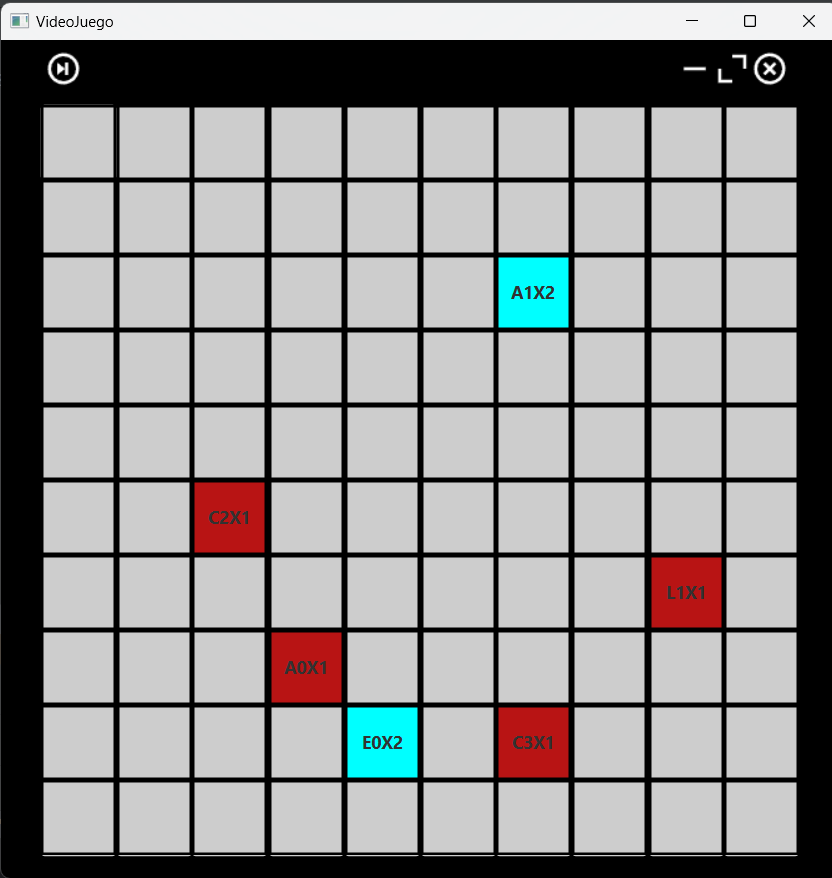
\includegraphics[width=0.6\textwidth,keepaspectratio]{img/tablero.png}
		%\includesvg{img/automata.svg}
		%\label{img:mot2}
		%\caption{Product backlog.}
	\end{figure}
	\begin{itemize}	
		\item Y con algunas capturas del funcionamiento del videojuego.
	\end{itemize}
	\begin{figure}[H]
		\centering
	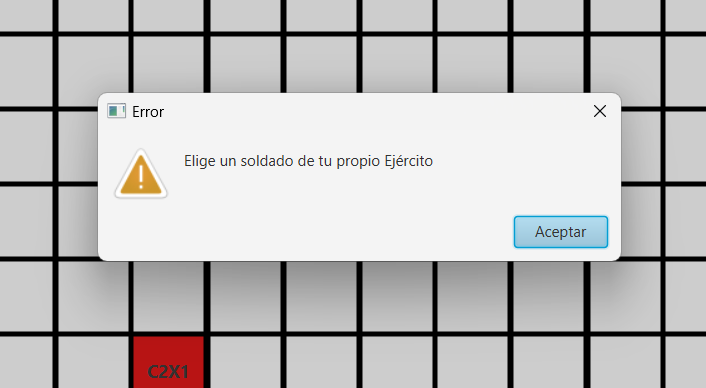
\includegraphics[width=0.6\textwidth,keepaspectratio]{img/menu1.png}
		%\includesvg{img/automata.svg}
		%\label{img:mot2}
		%\caption{Product backlog.}
	\end{figure}
	\begin{figure}[H]
		\centering
	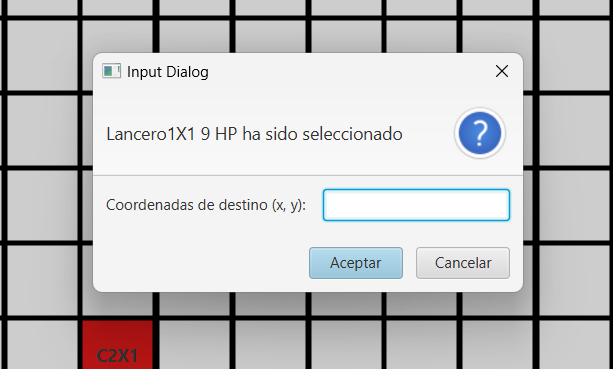
\includegraphics[width=0.6\textwidth,keepaspectratio]{img/menu2.png}
		%\includesvg{img/automata.svg}
		%\label{img:mot2}
		%\caption{Product backlog.}
	\end{figure}
	
	\begin{figure}[H]
		\centering
	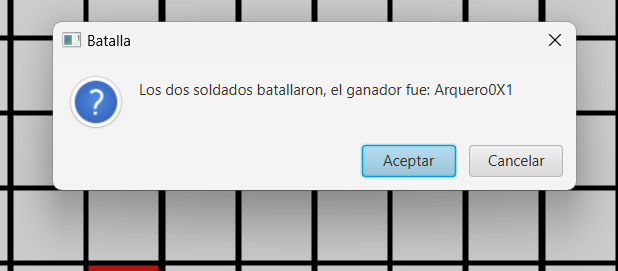
\includegraphics[width=0.6\textwidth,keepaspectratio]{img/menu3.png}
		%\includesvg{img/automata.svg}
		%\label{img:mot2}
		%\caption{Product backlog.}
	\end{figure}
	
	\begin{figure}[H]
		\centering
	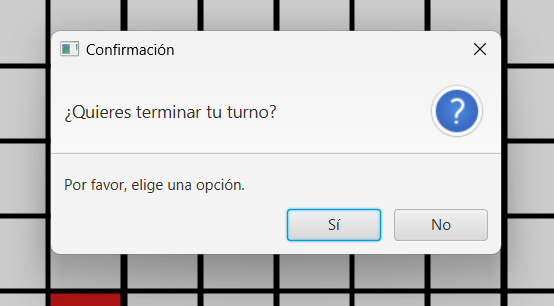
\includegraphics[width=0.6\textwidth,keepaspectratio]{img/menu4.png}
		%\includesvg{img/automata.svg}
		%\label{img:mot2}
		%\caption{Product backlog.}
	\end{figure}
	\begin{itemize}	
		\item Estos cambios fueron subidos al respositorio, a través de commits.
	\end{itemize}
	
	\begin{lstlisting}[language=bash,caption={Commit}, numbers=left][H]
	$commit feec5bf606898afbaaaadd1a80b1f0c0c356a83f (HEAD -> main, origin/main)
Author: RYAN VALDIVIA <rvaldiviase@unsa.edu.pe>
Date:   Sat Jan 20 11:48:31 2024 -0500

    Estableciendo las clases necesarias y realizando pruebas de JavaFx, usando IntelliJ Idea
	\end{lstlisting}
	
	\begin{lstlisting}[language=bash,caption={Commit}, numbers=left][H]
	$commit 44f6eaa51af046b665943d901d3ac65b04040216 (HEAD -> main, origin/main)
Author: RYAN VALDIVIA <rvaldiviase@unsa.edu.pe>
Date:   Mon Jan 22 13:38:31 2024 -0500

    Trabajo terminado, el juego es 100% funcional
	\end{lstlisting}
	
	\begin{itemize}	
		\item Además, aquí está el diagrama UML de todo el proyecto.
	\end{itemize}
	\begin{figure}[H]
		\centering
	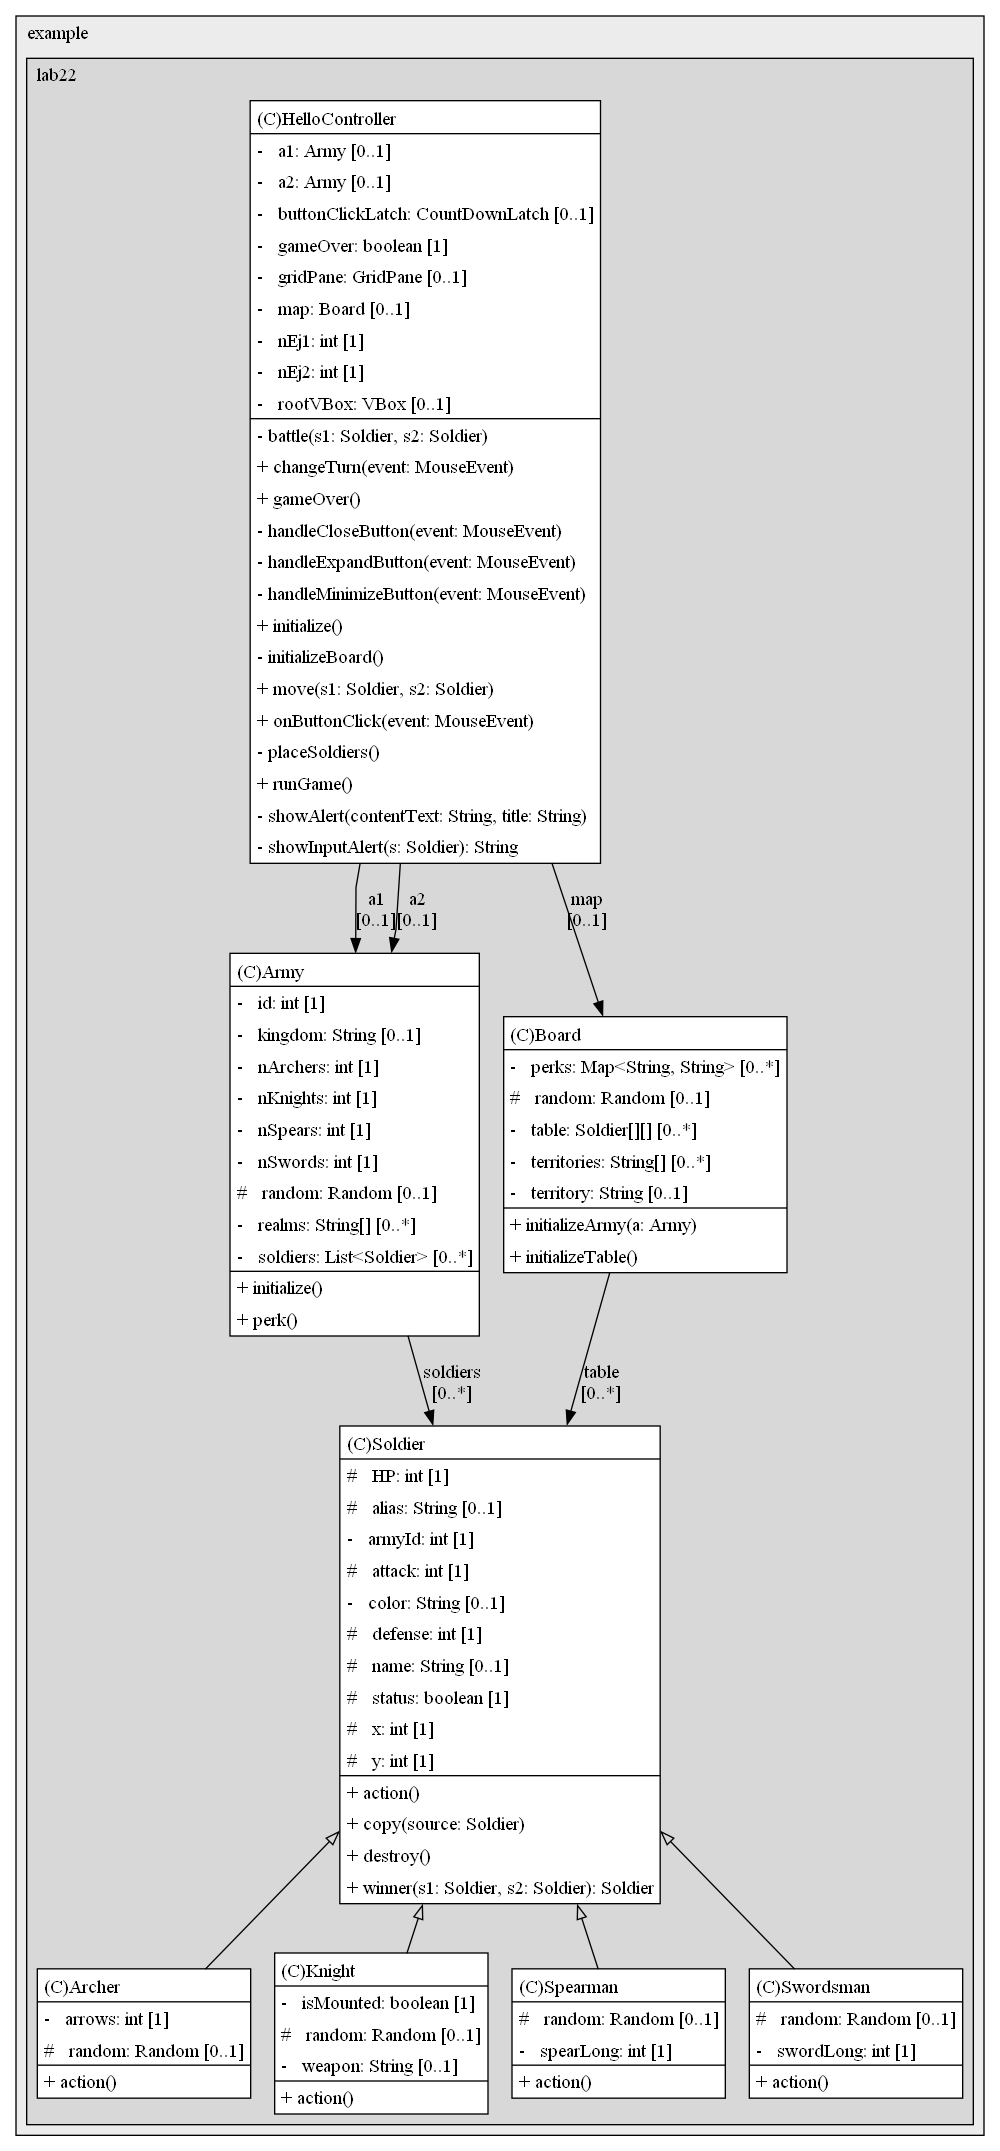
\includegraphics[width=0.6\textwidth,keepaspectratio]{img/HelloController_structure.png}
		%\includesvg{img/automata.svg}
		%\label{img:mot2}
		%\caption{Product backlog.}
	\end{figure}
	
	
	\section{\textcolor{red}{Rúbricas}}
	
	\subsection{\textcolor{red}{Entregable Informe}}
	\begin{table}[H]
		\caption{Tipo de Informe}
		\setlength{\tabcolsep}{0.5em} % for the horizontal padding
		{\renewcommand{\arraystretch}{1.5}% for the vertical padding
		\begin{tabular}{|p{3cm}|p{12cm}|}
			\hline
			\multicolumn{2}{|c|}{\textbf{\textcolor{red}{Informe}}}  \\
			\hline 
			\textbf{\textcolor{red}{Latex}} & \textcolor{blue}{El informe está en formato PDF desde Latex,  con un formato limpio (buena presentación) y facil de leer.}   \\ 
			\hline 
			
			
		\end{tabular}
	}
	\end{table}
	
	\clearpage
	
	\subsection{\textcolor{red}{Rúbrica para el contenido del Informe y demostración}}
	\begin{itemize}			
		\item El alumno debe marcar o dejar en blanco en celdas de la columna \textbf{Checklist} si cumplio con el ítem correspondiente.
		\item Si un alumno supera la fecha de entrega,  su calificación será sobre la nota mínima aprobada, siempre y cuando cumpla con todos lo items.
		\item El alumno debe autocalificarse en la columna \textbf{Estudiante} de acuerdo a la siguiente tabla:
	
		\begin{table}[ht]
			\caption{Niveles de desempeño}
			\begin{center}
			\begin{tabular}{ccccc}
    			\hline
    			 & \multicolumn{4}{c}{Nivel}\\
    			\cline{1-5}
    			\textbf{Puntos} & Insatisfactorio 25\%& En Proceso 50\% & Satisfactorio 75\% & Sobresaliente 100\%\\
    			\textbf{2.0}&0.5&1.0&1.5&2.0\\
    			\textbf{4.0}&1.0&2.0&3.0&4.0\\
    		\hline
			\end{tabular}
		\end{center}
	\end{table}	
	
	\end{itemize}
	
	\begin{table}[H]
		\caption{Rúbrica para contenido del Informe y demostración}
		\setlength{\tabcolsep}{0.5em} % for the horizontal padding
		{\renewcommand{\arraystretch}{1.5}% for the vertical padding
		%\begin{center}
		\begin{tabular}{|p{2.7cm}|p{7cm}|x{1.3cm}|p{1.2cm}|p{1.5cm}|p{1.1cm}|}
			\hline
    		\multicolumn{2}{|c|}{Contenido y demostración} & Puntos & Checklist & Estudiante & Profesor\\
			\hline
			\textbf{1. GitHub} & Hay enlace URL activo del directorio para el  laboratorio hacia su repositorio GitHub con código fuente terminado y fácil de revisar. &2 &X &2 & \\ 
			\hline
			\textbf{2. Commits} &  Hay capturas de pantalla de los commits más importantes con sus explicaciones detalladas. (El profesor puede preguntar para refrendar calificación). &4 &X &2 & \\ 
			\hline 
			\textbf{3. Código fuente} &  Hay porciones de código fuente importantes con numeración y explicaciones detalladas de sus funciones. &2 &X &2 & \\ 
			\hline 
			\textbf{4. Ejecución} & Se incluyen ejecuciones/pruebas del código fuente  explicadas gradualmente. &2 &X &2 & \\ 
			\hline			
			\textbf{5. Pregunta} & Se responde con completitud a la pregunta formulada en la tarea.  (El profesor puede preguntar para refrendar calificación).  &2 &X &2 & \\ 
			\hline	
			\textbf{6. Fechas} & Las fechas de modificación del código fuente estan dentro de los plazos de fecha de entrega establecidos. &2 &X &2 & \\ 
			\hline 
			\textbf{7. Ortografía} & El documento no muestra errores ortográficos. &2 &X &2 & \\ 
			\hline 
			\textbf{8. Madurez} & El Informe muestra de manera general una evolución de la madurez del código fuente,  explicaciones puntuales pero precisas y un acabado impecable.   (El profesor puede preguntar para refrendar calificación).  &4 &X &4 & \\ 
			\hline
			\multicolumn{2}{|c|}{\textbf{Total}} &20 & &18 & \\ 
			\hline
		\end{tabular}
		%\end{center}
		%\label{tab:multicol}
		}
	\end{table}
	
\clearpage

\section{Referencias}
	\begin{itemize}
		\item Fundamentos de la programación 2 - Tópicos de la programación Orientada a Objetos (Marco Aedo)
	\end{itemize}
	
%\clearpage
%\bibliographystyle{apalike}
%\bibliographystyle{IEEEtranN}
%\bibliography{bibliography}
			
\end{document}
